\documentclass[11pt]{article}

    \usepackage[breakable]{tcolorbox}
    \usepackage{parskip} % Stop auto-indenting (to mimic markdown behaviour)
    

    % Basic figure setup, for now with no caption control since it's done
    % automatically by Pandoc (which extracts ![](path) syntax from Markdown).
    \usepackage{graphicx}
    % Maintain compatibility with old templates. Remove in nbconvert 6.0
    \let\Oldincludegraphics\includegraphics
    % Ensure that by default, figures have no caption (until we provide a
    % proper Figure object with a Caption API and a way to capture that
    % in the conversion process - todo).
    \usepackage{caption}
    \DeclareCaptionFormat{nocaption}{}
    \captionsetup{format=nocaption,aboveskip=0pt,belowskip=0pt}

    \usepackage{float}
    \floatplacement{figure}{H} % forces figures to be placed at the correct location
    \usepackage{xcolor} % Allow colors to be defined
    \usepackage{enumerate} % Needed for markdown enumerations to work
    \usepackage{geometry} % Used to adjust the document margins
    \usepackage{amsmath} % Equations
    \usepackage{amssymb} % Equations
    \usepackage{textcomp} % defines textquotesingle
    % Hack from http://tex.stackexchange.com/a/47451/13684:
    \AtBeginDocument{%
        \def\PYZsq{\textquotesingle}% Upright quotes in Pygmentized code
    }
    \usepackage{upquote} % Upright quotes for verbatim code
    \usepackage{eurosym} % defines \euro

    \usepackage{iftex}
    \ifPDFTeX
        \usepackage[T1]{fontenc}
        \IfFileExists{alphabeta.sty}{
              \usepackage{alphabeta}
          }{
              \usepackage[mathletters]{ucs}
              \usepackage[utf8x]{inputenc}
          }
    \else
        \usepackage{fontspec}
        \usepackage{unicode-math}
    \fi

    \usepackage{fancyvrb} % verbatim replacement that allows latex
    \usepackage{grffile} % extends the file name processing of package graphics
                         % to support a larger range
    \makeatletter % fix for old versions of grffile with XeLaTeX
    \@ifpackagelater{grffile}{2019/11/01}
    {
      % Do nothing on new versions
    }
    {
      \def\Gread@@xetex#1{%
        \IfFileExists{"\Gin@base".bb}%
        {\Gread@eps{\Gin@base.bb}}%
        {\Gread@@xetex@aux#1}%
      }
    }
    \makeatother
    \usepackage[Export]{adjustbox} % Used to constrain images to a maximum size
    \adjustboxset{max size={0.9\linewidth}{0.9\paperheight}}

    % The hyperref package gives us a pdf with properly built
    % internal navigation ('pdf bookmarks' for the table of contents,
    % internal cross-reference links, web links for URLs, etc.)
    \usepackage{hyperref}
    % The default LaTeX title has an obnoxious amount of whitespace. By default,
    % titling removes some of it. It also provides customization options.
    \usepackage{titling}
    \usepackage{longtable} % longtable support required by pandoc >1.10
    \usepackage{booktabs}  % table support for pandoc > 1.12.2
    \usepackage{array}     % table support for pandoc >= 2.11.3
    \usepackage{calc}      % table minipage width calculation for pandoc >= 2.11.1
    \usepackage[inline]{enumitem} % IRkernel/repr support (it uses the enumerate* environment)
    \usepackage[normalem]{ulem} % ulem is needed to support strikethroughs (\sout)
                                % normalem makes italics be italics, not underlines
    \usepackage{soul}      % strikethrough (\st) support for pandoc >= 3.0.0
    \usepackage{mathrsfs}
    

    
    % Colors for the hyperref package
    \definecolor{urlcolor}{rgb}{0,.145,.698}
    \definecolor{linkcolor}{rgb}{.71,0.21,0.01}
    \definecolor{citecolor}{rgb}{.12,.54,.11}

    % ANSI colors
    \definecolor{ansi-black}{HTML}{3E424D}
    \definecolor{ansi-black-intense}{HTML}{282C36}
    \definecolor{ansi-red}{HTML}{E75C58}
    \definecolor{ansi-red-intense}{HTML}{B22B31}
    \definecolor{ansi-green}{HTML}{00A250}
    \definecolor{ansi-green-intense}{HTML}{007427}
    \definecolor{ansi-yellow}{HTML}{DDB62B}
    \definecolor{ansi-yellow-intense}{HTML}{B27D12}
    \definecolor{ansi-blue}{HTML}{208FFB}
    \definecolor{ansi-blue-intense}{HTML}{0065CA}
    \definecolor{ansi-magenta}{HTML}{D160C4}
    \definecolor{ansi-magenta-intense}{HTML}{A03196}
    \definecolor{ansi-cyan}{HTML}{60C6C8}
    \definecolor{ansi-cyan-intense}{HTML}{258F8F}
    \definecolor{ansi-white}{HTML}{C5C1B4}
    \definecolor{ansi-white-intense}{HTML}{A1A6B2}
    \definecolor{ansi-default-inverse-fg}{HTML}{FFFFFF}
    \definecolor{ansi-default-inverse-bg}{HTML}{000000}

    % common color for the border for error outputs.
    \definecolor{outerrorbackground}{HTML}{FFDFDF}

    % commands and environments needed by pandoc snippets
    % extracted from the output of `pandoc -s`
    \providecommand{\tightlist}{%
      \setlength{\itemsep}{0pt}\setlength{\parskip}{0pt}}
    \DefineVerbatimEnvironment{Highlighting}{Verbatim}{commandchars=\\\{\}}
    % Add ',fontsize=\small' for more characters per line
    \newenvironment{Shaded}{}{}
    \newcommand{\KeywordTok}[1]{\textcolor[rgb]{0.00,0.44,0.13}{\textbf{{#1}}}}
    \newcommand{\DataTypeTok}[1]{\textcolor[rgb]{0.56,0.13,0.00}{{#1}}}
    \newcommand{\DecValTok}[1]{\textcolor[rgb]{0.25,0.63,0.44}{{#1}}}
    \newcommand{\BaseNTok}[1]{\textcolor[rgb]{0.25,0.63,0.44}{{#1}}}
    \newcommand{\FloatTok}[1]{\textcolor[rgb]{0.25,0.63,0.44}{{#1}}}
    \newcommand{\CharTok}[1]{\textcolor[rgb]{0.25,0.44,0.63}{{#1}}}
    \newcommand{\StringTok}[1]{\textcolor[rgb]{0.25,0.44,0.63}{{#1}}}
    \newcommand{\CommentTok}[1]{\textcolor[rgb]{0.38,0.63,0.69}{\textit{{#1}}}}
    \newcommand{\OtherTok}[1]{\textcolor[rgb]{0.00,0.44,0.13}{{#1}}}
    \newcommand{\AlertTok}[1]{\textcolor[rgb]{1.00,0.00,0.00}{\textbf{{#1}}}}
    \newcommand{\FunctionTok}[1]{\textcolor[rgb]{0.02,0.16,0.49}{{#1}}}
    \newcommand{\RegionMarkerTok}[1]{{#1}}
    \newcommand{\ErrorTok}[1]{\textcolor[rgb]{1.00,0.00,0.00}{\textbf{{#1}}}}
    \newcommand{\NormalTok}[1]{{#1}}

    % Additional commands for more recent versions of Pandoc
    \newcommand{\ConstantTok}[1]{\textcolor[rgb]{0.53,0.00,0.00}{{#1}}}
    \newcommand{\SpecialCharTok}[1]{\textcolor[rgb]{0.25,0.44,0.63}{{#1}}}
    \newcommand{\VerbatimStringTok}[1]{\textcolor[rgb]{0.25,0.44,0.63}{{#1}}}
    \newcommand{\SpecialStringTok}[1]{\textcolor[rgb]{0.73,0.40,0.53}{{#1}}}
    \newcommand{\ImportTok}[1]{{#1}}
    \newcommand{\DocumentationTok}[1]{\textcolor[rgb]{0.73,0.13,0.13}{\textit{{#1}}}}
    \newcommand{\AnnotationTok}[1]{\textcolor[rgb]{0.38,0.63,0.69}{\textbf{\textit{{#1}}}}}
    \newcommand{\CommentVarTok}[1]{\textcolor[rgb]{0.38,0.63,0.69}{\textbf{\textit{{#1}}}}}
    \newcommand{\VariableTok}[1]{\textcolor[rgb]{0.10,0.09,0.49}{{#1}}}
    \newcommand{\ControlFlowTok}[1]{\textcolor[rgb]{0.00,0.44,0.13}{\textbf{{#1}}}}
    \newcommand{\OperatorTok}[1]{\textcolor[rgb]{0.40,0.40,0.40}{{#1}}}
    \newcommand{\BuiltInTok}[1]{{#1}}
    \newcommand{\ExtensionTok}[1]{{#1}}
    \newcommand{\PreprocessorTok}[1]{\textcolor[rgb]{0.74,0.48,0.00}{{#1}}}
    \newcommand{\AttributeTok}[1]{\textcolor[rgb]{0.49,0.56,0.16}{{#1}}}
    \newcommand{\InformationTok}[1]{\textcolor[rgb]{0.38,0.63,0.69}{\textbf{\textit{{#1}}}}}
    \newcommand{\WarningTok}[1]{\textcolor[rgb]{0.38,0.63,0.69}{\textbf{\textit{{#1}}}}}


    % Define a nice break command that doesn't care if a line doesn't already
    % exist.
    \def\br{\hspace*{\fill} \\* }
    % Math Jax compatibility definitions
    \def\gt{>}
    \def\lt{<}
    \let\Oldtex\TeX
    \let\Oldlatex\LaTeX
    \renewcommand{\TeX}{\textrm{\Oldtex}}
    \renewcommand{\LaTeX}{\textrm{\Oldlatex}}
    % Document parameters
    % Document title
    \title{Module7-HW}
    
    
    
    
    
    
    
% Pygments definitions
\makeatletter
\def\PY@reset{\let\PY@it=\relax \let\PY@bf=\relax%
    \let\PY@ul=\relax \let\PY@tc=\relax%
    \let\PY@bc=\relax \let\PY@ff=\relax}
\def\PY@tok#1{\csname PY@tok@#1\endcsname}
\def\PY@toks#1+{\ifx\relax#1\empty\else%
    \PY@tok{#1}\expandafter\PY@toks\fi}
\def\PY@do#1{\PY@bc{\PY@tc{\PY@ul{%
    \PY@it{\PY@bf{\PY@ff{#1}}}}}}}
\def\PY#1#2{\PY@reset\PY@toks#1+\relax+\PY@do{#2}}

\@namedef{PY@tok@w}{\def\PY@tc##1{\textcolor[rgb]{0.73,0.73,0.73}{##1}}}
\@namedef{PY@tok@c}{\let\PY@it=\textit\def\PY@tc##1{\textcolor[rgb]{0.24,0.48,0.48}{##1}}}
\@namedef{PY@tok@cp}{\def\PY@tc##1{\textcolor[rgb]{0.61,0.40,0.00}{##1}}}
\@namedef{PY@tok@k}{\let\PY@bf=\textbf\def\PY@tc##1{\textcolor[rgb]{0.00,0.50,0.00}{##1}}}
\@namedef{PY@tok@kp}{\def\PY@tc##1{\textcolor[rgb]{0.00,0.50,0.00}{##1}}}
\@namedef{PY@tok@kt}{\def\PY@tc##1{\textcolor[rgb]{0.69,0.00,0.25}{##1}}}
\@namedef{PY@tok@o}{\def\PY@tc##1{\textcolor[rgb]{0.40,0.40,0.40}{##1}}}
\@namedef{PY@tok@ow}{\let\PY@bf=\textbf\def\PY@tc##1{\textcolor[rgb]{0.67,0.13,1.00}{##1}}}
\@namedef{PY@tok@nb}{\def\PY@tc##1{\textcolor[rgb]{0.00,0.50,0.00}{##1}}}
\@namedef{PY@tok@nf}{\def\PY@tc##1{\textcolor[rgb]{0.00,0.00,1.00}{##1}}}
\@namedef{PY@tok@nc}{\let\PY@bf=\textbf\def\PY@tc##1{\textcolor[rgb]{0.00,0.00,1.00}{##1}}}
\@namedef{PY@tok@nn}{\let\PY@bf=\textbf\def\PY@tc##1{\textcolor[rgb]{0.00,0.00,1.00}{##1}}}
\@namedef{PY@tok@ne}{\let\PY@bf=\textbf\def\PY@tc##1{\textcolor[rgb]{0.80,0.25,0.22}{##1}}}
\@namedef{PY@tok@nv}{\def\PY@tc##1{\textcolor[rgb]{0.10,0.09,0.49}{##1}}}
\@namedef{PY@tok@no}{\def\PY@tc##1{\textcolor[rgb]{0.53,0.00,0.00}{##1}}}
\@namedef{PY@tok@nl}{\def\PY@tc##1{\textcolor[rgb]{0.46,0.46,0.00}{##1}}}
\@namedef{PY@tok@ni}{\let\PY@bf=\textbf\def\PY@tc##1{\textcolor[rgb]{0.44,0.44,0.44}{##1}}}
\@namedef{PY@tok@na}{\def\PY@tc##1{\textcolor[rgb]{0.41,0.47,0.13}{##1}}}
\@namedef{PY@tok@nt}{\let\PY@bf=\textbf\def\PY@tc##1{\textcolor[rgb]{0.00,0.50,0.00}{##1}}}
\@namedef{PY@tok@nd}{\def\PY@tc##1{\textcolor[rgb]{0.67,0.13,1.00}{##1}}}
\@namedef{PY@tok@s}{\def\PY@tc##1{\textcolor[rgb]{0.73,0.13,0.13}{##1}}}
\@namedef{PY@tok@sd}{\let\PY@it=\textit\def\PY@tc##1{\textcolor[rgb]{0.73,0.13,0.13}{##1}}}
\@namedef{PY@tok@si}{\let\PY@bf=\textbf\def\PY@tc##1{\textcolor[rgb]{0.64,0.35,0.47}{##1}}}
\@namedef{PY@tok@se}{\let\PY@bf=\textbf\def\PY@tc##1{\textcolor[rgb]{0.67,0.36,0.12}{##1}}}
\@namedef{PY@tok@sr}{\def\PY@tc##1{\textcolor[rgb]{0.64,0.35,0.47}{##1}}}
\@namedef{PY@tok@ss}{\def\PY@tc##1{\textcolor[rgb]{0.10,0.09,0.49}{##1}}}
\@namedef{PY@tok@sx}{\def\PY@tc##1{\textcolor[rgb]{0.00,0.50,0.00}{##1}}}
\@namedef{PY@tok@m}{\def\PY@tc##1{\textcolor[rgb]{0.40,0.40,0.40}{##1}}}
\@namedef{PY@tok@gh}{\let\PY@bf=\textbf\def\PY@tc##1{\textcolor[rgb]{0.00,0.00,0.50}{##1}}}
\@namedef{PY@tok@gu}{\let\PY@bf=\textbf\def\PY@tc##1{\textcolor[rgb]{0.50,0.00,0.50}{##1}}}
\@namedef{PY@tok@gd}{\def\PY@tc##1{\textcolor[rgb]{0.63,0.00,0.00}{##1}}}
\@namedef{PY@tok@gi}{\def\PY@tc##1{\textcolor[rgb]{0.00,0.52,0.00}{##1}}}
\@namedef{PY@tok@gr}{\def\PY@tc##1{\textcolor[rgb]{0.89,0.00,0.00}{##1}}}
\@namedef{PY@tok@ge}{\let\PY@it=\textit}
\@namedef{PY@tok@gs}{\let\PY@bf=\textbf}
\@namedef{PY@tok@gp}{\let\PY@bf=\textbf\def\PY@tc##1{\textcolor[rgb]{0.00,0.00,0.50}{##1}}}
\@namedef{PY@tok@go}{\def\PY@tc##1{\textcolor[rgb]{0.44,0.44,0.44}{##1}}}
\@namedef{PY@tok@gt}{\def\PY@tc##1{\textcolor[rgb]{0.00,0.27,0.87}{##1}}}
\@namedef{PY@tok@err}{\def\PY@bc##1{{\setlength{\fboxsep}{\string -\fboxrule}\fcolorbox[rgb]{1.00,0.00,0.00}{1,1,1}{\strut ##1}}}}
\@namedef{PY@tok@kc}{\let\PY@bf=\textbf\def\PY@tc##1{\textcolor[rgb]{0.00,0.50,0.00}{##1}}}
\@namedef{PY@tok@kd}{\let\PY@bf=\textbf\def\PY@tc##1{\textcolor[rgb]{0.00,0.50,0.00}{##1}}}
\@namedef{PY@tok@kn}{\let\PY@bf=\textbf\def\PY@tc##1{\textcolor[rgb]{0.00,0.50,0.00}{##1}}}
\@namedef{PY@tok@kr}{\let\PY@bf=\textbf\def\PY@tc##1{\textcolor[rgb]{0.00,0.50,0.00}{##1}}}
\@namedef{PY@tok@bp}{\def\PY@tc##1{\textcolor[rgb]{0.00,0.50,0.00}{##1}}}
\@namedef{PY@tok@fm}{\def\PY@tc##1{\textcolor[rgb]{0.00,0.00,1.00}{##1}}}
\@namedef{PY@tok@vc}{\def\PY@tc##1{\textcolor[rgb]{0.10,0.09,0.49}{##1}}}
\@namedef{PY@tok@vg}{\def\PY@tc##1{\textcolor[rgb]{0.10,0.09,0.49}{##1}}}
\@namedef{PY@tok@vi}{\def\PY@tc##1{\textcolor[rgb]{0.10,0.09,0.49}{##1}}}
\@namedef{PY@tok@vm}{\def\PY@tc##1{\textcolor[rgb]{0.10,0.09,0.49}{##1}}}
\@namedef{PY@tok@sa}{\def\PY@tc##1{\textcolor[rgb]{0.73,0.13,0.13}{##1}}}
\@namedef{PY@tok@sb}{\def\PY@tc##1{\textcolor[rgb]{0.73,0.13,0.13}{##1}}}
\@namedef{PY@tok@sc}{\def\PY@tc##1{\textcolor[rgb]{0.73,0.13,0.13}{##1}}}
\@namedef{PY@tok@dl}{\def\PY@tc##1{\textcolor[rgb]{0.73,0.13,0.13}{##1}}}
\@namedef{PY@tok@s2}{\def\PY@tc##1{\textcolor[rgb]{0.73,0.13,0.13}{##1}}}
\@namedef{PY@tok@sh}{\def\PY@tc##1{\textcolor[rgb]{0.73,0.13,0.13}{##1}}}
\@namedef{PY@tok@s1}{\def\PY@tc##1{\textcolor[rgb]{0.73,0.13,0.13}{##1}}}
\@namedef{PY@tok@mb}{\def\PY@tc##1{\textcolor[rgb]{0.40,0.40,0.40}{##1}}}
\@namedef{PY@tok@mf}{\def\PY@tc##1{\textcolor[rgb]{0.40,0.40,0.40}{##1}}}
\@namedef{PY@tok@mh}{\def\PY@tc##1{\textcolor[rgb]{0.40,0.40,0.40}{##1}}}
\@namedef{PY@tok@mi}{\def\PY@tc##1{\textcolor[rgb]{0.40,0.40,0.40}{##1}}}
\@namedef{PY@tok@il}{\def\PY@tc##1{\textcolor[rgb]{0.40,0.40,0.40}{##1}}}
\@namedef{PY@tok@mo}{\def\PY@tc##1{\textcolor[rgb]{0.40,0.40,0.40}{##1}}}
\@namedef{PY@tok@ch}{\let\PY@it=\textit\def\PY@tc##1{\textcolor[rgb]{0.24,0.48,0.48}{##1}}}
\@namedef{PY@tok@cm}{\let\PY@it=\textit\def\PY@tc##1{\textcolor[rgb]{0.24,0.48,0.48}{##1}}}
\@namedef{PY@tok@cpf}{\let\PY@it=\textit\def\PY@tc##1{\textcolor[rgb]{0.24,0.48,0.48}{##1}}}
\@namedef{PY@tok@c1}{\let\PY@it=\textit\def\PY@tc##1{\textcolor[rgb]{0.24,0.48,0.48}{##1}}}
\@namedef{PY@tok@cs}{\let\PY@it=\textit\def\PY@tc##1{\textcolor[rgb]{0.24,0.48,0.48}{##1}}}

\def\PYZbs{\char`\\}
\def\PYZus{\char`\_}
\def\PYZob{\char`\{}
\def\PYZcb{\char`\}}
\def\PYZca{\char`\^}
\def\PYZam{\char`\&}
\def\PYZlt{\char`\<}
\def\PYZgt{\char`\>}
\def\PYZsh{\char`\#}
\def\PYZpc{\char`\%}
\def\PYZdl{\char`\$}
\def\PYZhy{\char`\-}
\def\PYZsq{\char`\'}
\def\PYZdq{\char`\"}
\def\PYZti{\char`\~}
% for compatibility with earlier versions
\def\PYZat{@}
\def\PYZlb{[}
\def\PYZrb{]}
\makeatother


    % For linebreaks inside Verbatim environment from package fancyvrb.
    \makeatletter
        \newbox\Wrappedcontinuationbox
        \newbox\Wrappedvisiblespacebox
        \newcommand*\Wrappedvisiblespace {\textcolor{red}{\textvisiblespace}}
        \newcommand*\Wrappedcontinuationsymbol {\textcolor{red}{\llap{\tiny$\m@th\hookrightarrow$}}}
        \newcommand*\Wrappedcontinuationindent {3ex }
        \newcommand*\Wrappedafterbreak {\kern\Wrappedcontinuationindent\copy\Wrappedcontinuationbox}
        % Take advantage of the already applied Pygments mark-up to insert
        % potential linebreaks for TeX processing.
        %        {, <, #, %, $, ' and ": go to next line.
        %        _, }, ^, &, >, - and ~: stay at end of broken line.
        % Use of \textquotesingle for straight quote.
        \newcommand*\Wrappedbreaksatspecials {%
            \def\PYGZus{\discretionary{\char`\_}{\Wrappedafterbreak}{\char`\_}}%
            \def\PYGZob{\discretionary{}{\Wrappedafterbreak\char`\{}{\char`\{}}%
            \def\PYGZcb{\discretionary{\char`\}}{\Wrappedafterbreak}{\char`\}}}%
            \def\PYGZca{\discretionary{\char`\^}{\Wrappedafterbreak}{\char`\^}}%
            \def\PYGZam{\discretionary{\char`\&}{\Wrappedafterbreak}{\char`\&}}%
            \def\PYGZlt{\discretionary{}{\Wrappedafterbreak\char`\<}{\char`\<}}%
            \def\PYGZgt{\discretionary{\char`\>}{\Wrappedafterbreak}{\char`\>}}%
            \def\PYGZsh{\discretionary{}{\Wrappedafterbreak\char`\#}{\char`\#}}%
            \def\PYGZpc{\discretionary{}{\Wrappedafterbreak\char`\%}{\char`\%}}%
            \def\PYGZdl{\discretionary{}{\Wrappedafterbreak\char`\$}{\char`\$}}%
            \def\PYGZhy{\discretionary{\char`\-}{\Wrappedafterbreak}{\char`\-}}%
            \def\PYGZsq{\discretionary{}{\Wrappedafterbreak\textquotesingle}{\textquotesingle}}%
            \def\PYGZdq{\discretionary{}{\Wrappedafterbreak\char`\"}{\char`\"}}%
            \def\PYGZti{\discretionary{\char`\~}{\Wrappedafterbreak}{\char`\~}}%
        }
        % Some characters . , ; ? ! / are not pygmentized.
        % This macro makes them "active" and they will insert potential linebreaks
        \newcommand*\Wrappedbreaksatpunct {%
            \lccode`\~`\.\lowercase{\def~}{\discretionary{\hbox{\char`\.}}{\Wrappedafterbreak}{\hbox{\char`\.}}}%
            \lccode`\~`\,\lowercase{\def~}{\discretionary{\hbox{\char`\,}}{\Wrappedafterbreak}{\hbox{\char`\,}}}%
            \lccode`\~`\;\lowercase{\def~}{\discretionary{\hbox{\char`\;}}{\Wrappedafterbreak}{\hbox{\char`\;}}}%
            \lccode`\~`\:\lowercase{\def~}{\discretionary{\hbox{\char`\:}}{\Wrappedafterbreak}{\hbox{\char`\:}}}%
            \lccode`\~`\?\lowercase{\def~}{\discretionary{\hbox{\char`\?}}{\Wrappedafterbreak}{\hbox{\char`\?}}}%
            \lccode`\~`\!\lowercase{\def~}{\discretionary{\hbox{\char`\!}}{\Wrappedafterbreak}{\hbox{\char`\!}}}%
            \lccode`\~`\/\lowercase{\def~}{\discretionary{\hbox{\char`\/}}{\Wrappedafterbreak}{\hbox{\char`\/}}}%
            \catcode`\.\active
            \catcode`\,\active
            \catcode`\;\active
            \catcode`\:\active
            \catcode`\?\active
            \catcode`\!\active
            \catcode`\/\active
            \lccode`\~`\~
        }
    \makeatother

    \let\OriginalVerbatim=\Verbatim
    \makeatletter
    \renewcommand{\Verbatim}[1][1]{%
        %\parskip\z@skip
        \sbox\Wrappedcontinuationbox {\Wrappedcontinuationsymbol}%
        \sbox\Wrappedvisiblespacebox {\FV@SetupFont\Wrappedvisiblespace}%
        \def\FancyVerbFormatLine ##1{\hsize\linewidth
            \vtop{\raggedright\hyphenpenalty\z@\exhyphenpenalty\z@
                \doublehyphendemerits\z@\finalhyphendemerits\z@
                \strut ##1\strut}%
        }%
        % If the linebreak is at a space, the latter will be displayed as visible
        % space at end of first line, and a continuation symbol starts next line.
        % Stretch/shrink are however usually zero for typewriter font.
        \def\FV@Space {%
            \nobreak\hskip\z@ plus\fontdimen3\font minus\fontdimen4\font
            \discretionary{\copy\Wrappedvisiblespacebox}{\Wrappedafterbreak}
            {\kern\fontdimen2\font}%
        }%

        % Allow breaks at special characters using \PYG... macros.
        \Wrappedbreaksatspecials
        % Breaks at punctuation characters . , ; ? ! and / need catcode=\active
        \OriginalVerbatim[#1,codes*=\Wrappedbreaksatpunct]%
    }
    \makeatother

    % Exact colors from NB
    \definecolor{incolor}{HTML}{303F9F}
    \definecolor{outcolor}{HTML}{D84315}
    \definecolor{cellborder}{HTML}{CFCFCF}
    \definecolor{cellbackground}{HTML}{F7F7F7}

    % prompt
    \makeatletter
    \newcommand{\boxspacing}{\kern\kvtcb@left@rule\kern\kvtcb@boxsep}
    \makeatother
    \newcommand{\prompt}[4]{
        {\ttfamily\llap{{\color{#2}[#3]:\hspace{3pt}#4}}\vspace{-\baselineskip}}
    }
    

    
    % Prevent overflowing lines due to hard-to-break entities
    \sloppy
    % Setup hyperref package
    \hypersetup{
      breaklinks=true,  % so long urls are correctly broken across lines
      colorlinks=true,
      urlcolor=urlcolor,
      linkcolor=linkcolor,
      citecolor=citecolor,
      }
    % Slightly bigger margins than the latex defaults
    
    \geometry{verbose,tmargin=1in,bmargin=1in,lmargin=1in,rmargin=1in}
    
    

\begin{document}
    
    \maketitle
    
    

    
    \textbf{Problem1-LeetcodeQ 703-Kth Largest Element in a Stream-Easy}

Design a class to find the kth largest element in a stream. Note that it
is the kth largest element in the sorted order, not the kth distinct
element.

Implement KthLargest class:

KthLargest(int k, int{[}{]} nums) Initializes the object with the
integer k and the stream of integers nums. int add(int val) Appends the
integer val to the stream and returns the element representing the kth
largest element in the stream.

\textbf{Example 1:}

\begin{itemize}
\item
  Input

  \begin{itemize}
  \tightlist
  \item
    {[}``KthLargest'', ``add'', ``add'', ``add'', ``add'', ``add''{]}
  \item
    {[}{[}3, {[}4, 5, 8, 2{]}{]}, {[}3{]}, {[}5{]}, {[}10{]}, {[}9{]},
    {[}4{]}{]}
  \end{itemize}
\item
  Output

  \begin{itemize}
  \tightlist
  \item
    {[}null, 4, 5, 5, 8, 8{]}
  \end{itemize}
\item
  Explanation -KthLargest kthLargest = new KthLargest(3, {[}4, 5, 8,
  2{]}); -kthLargest.add(3); // return 4 -kthLargest.add(5); // return 5
  -kthLargest.add(10); // return 5 -kthLargest.add(9); // return 8
  -kthLargest.add(4); // return 8
\item
  Constraints:

  \begin{itemize}
  \tightlist
  \item
    1 \textless= k \textless= 104
  \item
    0 \textless= nums.length \textless= 104
  \item
    -104 \textless= nums{[}i{]} \textless= 104
  \item
    -104 \textless= val \textless= 104
  \item
    At most 104 calls will be made to add.
  \item
    It is guaranteed that there will be at least k elements in the array
    when you search for the kth element.
  \end{itemize}
\end{itemize}

    \subsubsection{Q703 Psuedocode}\label{q703-psuedocode}

    \begin{tcolorbox}[breakable, size=fbox, boxrule=1pt, pad at break*=1mm,colback=cellbackground, colframe=cellborder]
\prompt{In}{incolor}{ }{\boxspacing}
\begin{Verbatim}[commandchars=\\\{\}]
\PY{n}{initialize}\PY{p}{:}
    \PY{o}{\PYZhy{}} \PY{n}{k} \PY{k}{as} \PY{n}{integer}
    \PY{o}{\PYZhy{}} \PY{n}{heap} \PY{k}{as} \PY{n}{empty} \PY{n+nb}{list}
    \PY{n}{For} \PY{n}{each} \PY{n}{num} \PY{o+ow}{in} \PY{n}{nums}\PY{p}{:}
        \PY{n}{Push} \PY{n}{num} \PY{n}{into} \PY{n}{heap}
        \PY{n}{If} \PY{n}{size} \PY{n}{of} \PY{n}{heap} \PY{o+ow}{is} \PY{n}{greater} \PY{n}{than} \PY{n}{k}\PY{p}{:}
            \PY{n}{Pop} \PY{n}{smallest} \PY{n}{element} \PY{k+kn}{from} \PY{n+nn}{heap}

\PY{n}{function} \PY{n}{add}\PY{p}{(}\PY{n}{val}\PY{p}{)}\PY{p}{:}
    \PY{n}{Push} \PY{n}{val} \PY{n}{into} \PY{n}{heap}
    \PY{n}{If} \PY{n}{size} \PY{n}{of} \PY{n}{heap} \PY{o+ow}{is} \PY{n}{greater} \PY{n}{than} \PY{n}{k}\PY{p}{:}
        \PY{n}{Pop} \PY{n}{smallest} \PY{n}{element} \PY{k+kn}{from} \PY{n+nn}{heap}
    \PY{n}{Return} \PY{n}{smallest} \PY{n}{element} \PY{k+kn}{from} \PY{n+nn}{heap} \PY{p}{(}\PY{n}{which} \PY{o+ow}{is} \PY{n}{heap}\PY{p}{[}\PY{l+m+mi}{0}\PY{p}{]}\PY{p}{)}
\end{Verbatim}
\end{tcolorbox}

    \subsubsection{Q703 Code.py}\label{q703-code.py}

    \begin{tcolorbox}[breakable, size=fbox, boxrule=1pt, pad at break*=1mm,colback=cellbackground, colframe=cellborder]
\prompt{In}{incolor}{4}{\boxspacing}
\begin{Verbatim}[commandchars=\\\{\}]
\PY{k+kn}{from} \PY{n+nn}{typing} \PY{k+kn}{import} \PY{n}{List}
\PY{k+kn}{import} \PY{n+nn}{heapq}

\PY{k}{class} \PY{n+nc}{KthLargest}\PY{p}{:}
    \PY{k}{def} \PY{n+nf+fm}{\PYZus{}\PYZus{}init\PYZus{}\PYZus{}}\PY{p}{(}\PY{n+nb+bp}{self}\PY{p}{,} \PY{n}{k}\PY{p}{:} \PY{n+nb}{int}\PY{p}{,} \PY{n}{nums}\PY{p}{:} \PY{n}{List}\PY{p}{[}\PY{n+nb}{int}\PY{p}{]}\PY{p}{)}\PY{p}{:}
        \PY{n+nb+bp}{self}\PY{o}{.}\PY{n}{heap} \PY{o}{=} \PY{p}{[}\PY{p}{]}
        \PY{n+nb+bp}{self}\PY{o}{.}\PY{n}{k} \PY{o}{=} \PY{n}{k}
        \PY{k}{for} \PY{n}{num} \PY{o+ow}{in} \PY{n}{nums}\PY{p}{:}
            \PY{n}{heapq}\PY{o}{.}\PY{n}{heappush}\PY{p}{(}\PY{n+nb+bp}{self}\PY{o}{.}\PY{n}{heap}\PY{p}{,} \PY{n}{num}\PY{p}{)}
            \PY{k}{if} \PY{n+nb}{len}\PY{p}{(}\PY{n+nb+bp}{self}\PY{o}{.}\PY{n}{heap}\PY{p}{)} \PY{o}{\PYZgt{}} \PY{n}{k}\PY{p}{:}
                \PY{n}{heapq}\PY{o}{.}\PY{n}{heappop}\PY{p}{(}\PY{n+nb+bp}{self}\PY{o}{.}\PY{n}{heap}\PY{p}{)}

    \PY{k}{def} \PY{n+nf}{add}\PY{p}{(}\PY{n+nb+bp}{self}\PY{p}{,} \PY{n}{val}\PY{p}{:} \PY{n+nb}{int}\PY{p}{)} \PY{o}{\PYZhy{}}\PY{o}{\PYZgt{}} \PY{n+nb}{int}\PY{p}{:}
        \PY{n}{heapq}\PY{o}{.}\PY{n}{heappush}\PY{p}{(}\PY{n+nb+bp}{self}\PY{o}{.}\PY{n}{heap}\PY{p}{,} \PY{n}{val}\PY{p}{)}
        \PY{k}{if} \PY{n+nb}{len}\PY{p}{(}\PY{n+nb+bp}{self}\PY{o}{.}\PY{n}{heap}\PY{p}{)} \PY{o}{\PYZgt{}} \PY{n+nb+bp}{self}\PY{o}{.}\PY{n}{k}\PY{p}{:}
            \PY{n}{heapq}\PY{o}{.}\PY{n}{heappop}\PY{p}{(}\PY{n+nb+bp}{self}\PY{o}{.}\PY{n}{heap}\PY{p}{)}
        \PY{k}{return} \PY{n+nb+bp}{self}\PY{o}{.}\PY{n}{heap}\PY{p}{[}\PY{l+m+mi}{0}\PY{p}{]}


\PY{n}{kth\PYZus{}largest} \PY{o}{=} \PY{n}{KthLargest}\PY{p}{(}\PY{l+m+mi}{3}\PY{p}{,} \PY{p}{[}\PY{l+m+mi}{4}\PY{p}{,} \PY{l+m+mi}{5}\PY{p}{,} \PY{l+m+mi}{8}\PY{p}{,} \PY{l+m+mi}{2}\PY{p}{]}\PY{p}{)}
\PY{n+nb}{print}\PY{p}{(}\PY{n}{kth\PYZus{}largest}\PY{o}{.}\PY{n}{add}\PY{p}{(}\PY{l+m+mi}{3}\PY{p}{)}\PY{p}{)}  \PY{c+c1}{\PYZsh{} Output: 4}
\PY{n+nb}{print}\PY{p}{(}\PY{n}{kth\PYZus{}largest}\PY{o}{.}\PY{n}{add}\PY{p}{(}\PY{l+m+mi}{5}\PY{p}{)}\PY{p}{)}  \PY{c+c1}{\PYZsh{} Output: 5}
\PY{n+nb}{print}\PY{p}{(}\PY{n}{kth\PYZus{}largest}\PY{o}{.}\PY{n}{add}\PY{p}{(}\PY{l+m+mi}{10}\PY{p}{)}\PY{p}{)}  \PY{c+c1}{\PYZsh{} Output: 5}
\PY{n+nb}{print}\PY{p}{(}\PY{n}{kth\PYZus{}largest}\PY{o}{.}\PY{n}{add}\PY{p}{(}\PY{l+m+mi}{9}\PY{p}{)}\PY{p}{)}  \PY{c+c1}{\PYZsh{} Output: 8}
\PY{n+nb}{print}\PY{p}{(}\PY{n}{kth\PYZus{}largest}\PY{o}{.}\PY{n}{add}\PY{p}{(}\PY{l+m+mi}{4}\PY{p}{)}\PY{p}{)}  \PY{c+c1}{\PYZsh{} Output: 8}
\end{Verbatim}
\end{tcolorbox}

    \begin{Verbatim}[commandchars=\\\{\}]
4
5
5
8
8
    \end{Verbatim}

    \textbf{Problem2-LeetcodeQ 1046- Last Stone Weight-Easy}

You are given an array of integers stones where stones{[}i{]} is the
weight of the ith stone.

We are playing a game with the stones. On each turn, we choose the
heaviest two stones and smash them together. Suppose the heaviest two
stones have weights x and y with x \textless= y. The result of this
smash is:

If x == y, both stones are destroyed, and If x != y, the stone of weight
x is destroyed, and the stone of weight y has new weight y - x. At the
end of the game, there is at most one stone left.

Return the weight of the last remaining stone. If there are no stones
left, return 0.

\begin{itemize}
\item
  Example 1:

  \begin{itemize}
  \tightlist
  \item
    Input: stones = {[}2,7,4,1,8,1{]}
  \item
    Output: 1
  \end{itemize}
\item
  Explanation:

  \begin{itemize}
  \tightlist
  \item
    We combine 7 and 8 to get 1 so the array converts to {[}2,4,1,1,1{]}
    then,
  \item
    we combine 2 and 4 to get 2 so the array converts to {[}2,1,1,1{]}
    then,
  \item
    we combine 2 and 1 to get 1 so the array converts to {[}1,1,1{]}
    then,
  \item
    we combine 1 and 1 to get 0 so the array converts to {[}1{]} then
    that's the value of the last stone.
  \end{itemize}
\item
  Example 2:

  \begin{itemize}
  \tightlist
  \item
    Input: stones = {[}1{]}
  \item
    Output: 1
  \end{itemize}
\item
  Constraints:

  \begin{itemize}
  \tightlist
  \item
    1 \textless= stones.length \textless= 30
  \item
    1 \textless= stones{[}i{]} \textless= 1000
  \end{itemize}
\end{itemize}

    \subsubsection{Q1046 Psuedocode}\label{q1046-psuedocode}

    \begin{tcolorbox}[breakable, size=fbox, boxrule=1pt, pad at break*=1mm,colback=cellbackground, colframe=cellborder]
\prompt{In}{incolor}{ }{\boxspacing}
\begin{Verbatim}[commandchars=\\\{\}]
\PY{n}{function} \PY{n}{last\PYZus{}stone\PYZus{}weight}\PY{p}{(}\PY{n}{stones}\PY{p}{)}\PY{p}{:}
\PY{n}{Create} \PY{n}{a} \PY{n+nb}{max} \PY{n}{heap} \PY{n}{of} \PY{n}{negative} \PY{n}{values} \PY{n}{of} \PY{n}{stone} \PY{n}{heap} \PY{o}{=} \PY{p}{[}\PY{p}{]}
\PY{k}{for} \PY{n}{stone} \PY{o+ow}{in} \PY{n}{stones}\PY{p}{:}
    \PY{n}{heap}\PY{o}{.}\PY{n}{push}\PY{p}{(}\PY{o}{\PYZhy{}}\PY{n}{stone}\PY{p}{)}

\PY{n}{Convert} \PY{n}{the} \PY{n+nb}{list} \PY{n}{into} \PY{n}{a} \PY{n}{heap} \PY{o+ow}{in}\PY{o}{\PYZhy{}}\PY{n}{place} \PY{n}{heapify}\PY{p}{(}\PY{n}{heap}\PY{p}{)}  

\PY{n}{While} \PY{n}{there} \PY{n}{are} \PY{n}{more} \PY{n}{than} \PY{l+m+mi}{1} \PY{n}{stone} \PY{n}{left} \PY{o+ow}{in} \PY{n}{the} \PY{n}{heap}

\PY{n}{Extract} \PY{n}{the} \PY{n}{two} \PY{n}{largest} \PY{n}{stones} \PY{p}{(}\PY{o+ow}{in} \PY{n}{negative} \PY{n}{form}\PY{p}{)}
\PY{n}{If} \PY{n}{they} \PY{n}{are} \PY{o+ow}{not} \PY{n}{equal}\PY{p}{,} \PY{n}{smash} \PY{n}{them} \PY{o+ow}{and} \PY{n}{push} \PY{n}{the} \PY{n}{difference} \PY{n}{back} \PY{n}{to} \PY{n}{the} \PY{n}{heap}
\PY{n}{If} \PY{n}{there} \PY{o+ow}{is} \PY{n}{one} \PY{n}{stone} \PY{n}{left}\PY{p}{,} \PY{k}{return} \PY{n}{its} \PY{n}{weight} \PY{p}{(}\PY{n}{convert} \PY{n}{back} \PY{k+kn}{from} \PY{n+nn}{negative}\PY{p}{)}
\PY{n}{If} \PY{n}{no} \PY{n}{stones} \PY{n}{are} \PY{n}{left}\PY{p}{,} \PY{k}{return} \PY{l+m+mi}{0}
\end{Verbatim}
\end{tcolorbox}

    \subsubsection{Q1046 Code.py}\label{q1046-code.py}

    \begin{tcolorbox}[breakable, size=fbox, boxrule=1pt, pad at break*=1mm,colback=cellbackground, colframe=cellborder]
\prompt{In}{incolor}{9}{\boxspacing}
\begin{Verbatim}[commandchars=\\\{\}]
\PY{k+kn}{import} \PY{n+nn}{heapq}

\PY{k}{class} \PY{n+nc}{Solution}\PY{p}{:}
    \PY{k}{def} \PY{n+nf}{last\PYZus{}stone\PYZus{}weight}\PY{p}{(}\PY{n+nb+bp}{self}\PY{p}{,} \PY{n}{stones}\PY{p}{)}\PY{p}{:}
        \PY{n}{heap} \PY{o}{=} \PY{p}{[}\PY{o}{\PYZhy{}}\PY{n}{stone} \PY{k}{for} \PY{n}{stone} \PY{o+ow}{in} \PY{n}{stones}\PY{p}{]}  
        \PY{n}{heapq}\PY{o}{.}\PY{n}{heapify}\PY{p}{(}\PY{n}{heap}\PY{p}{)} 

        \PY{k}{while} \PY{n+nb}{len}\PY{p}{(}\PY{n}{heap}\PY{p}{)} \PY{o}{\PYZgt{}} \PY{l+m+mi}{1}\PY{p}{:}
            \PY{n}{x} \PY{o}{=} \PY{n}{heapq}\PY{o}{.}\PY{n}{heappop}\PY{p}{(}\PY{n}{heap}\PY{p}{)}  
            \PY{n}{y} \PY{o}{=} \PY{n}{heapq}\PY{o}{.}\PY{n}{heappop}\PY{p}{(}\PY{n}{heap}\PY{p}{)}  

            \PY{k}{if} \PY{n}{x} \PY{o}{!=} \PY{n}{y}\PY{p}{:}
                \PY{n}{heapq}\PY{o}{.}\PY{n}{heappush}\PY{p}{(}\PY{n}{heap}\PY{p}{,} \PY{n}{x} \PY{o}{\PYZhy{}} \PY{n}{y}\PY{p}{)} 

        \PY{k}{if} \PY{n}{heap}\PY{p}{:}
            \PY{k}{return} \PY{o}{\PYZhy{}}\PY{n}{heap}\PY{p}{[}\PY{l+m+mi}{0}\PY{p}{]}  
        \PY{k}{else}\PY{p}{:}
            \PY{k}{return} \PY{l+m+mi}{0}  

\PY{n}{solution} \PY{o}{=} \PY{n}{Solution}\PY{p}{(}\PY{p}{)}
\PY{n}{stones} \PY{o}{=} \PY{p}{[}\PY{l+m+mi}{2}\PY{p}{,} \PY{l+m+mi}{7}\PY{p}{,} \PY{l+m+mi}{4}\PY{p}{,} \PY{l+m+mi}{1}\PY{p}{,} \PY{l+m+mi}{8}\PY{p}{,} \PY{l+m+mi}{1}\PY{p}{]}
\PY{n+nb}{print}\PY{p}{(}\PY{n}{solution}\PY{o}{.}\PY{n}{last\PYZus{}stone\PYZus{}weight}\PY{p}{(}\PY{n}{stones}\PY{p}{)}\PY{p}{)} 
\end{Verbatim}
\end{tcolorbox}

    \begin{Verbatim}[commandchars=\\\{\}]
1
    \end{Verbatim}

    \begin{tcolorbox}[breakable, size=fbox, boxrule=1pt, pad at break*=1mm,colback=cellbackground, colframe=cellborder]
\prompt{In}{incolor}{ }{\boxspacing}
\begin{Verbatim}[commandchars=\\\{\}]

\end{Verbatim}
\end{tcolorbox}

    \textbf{Problem3-LeetcodeQ 973. K Closest Points to Origin-Medium}

Given an array of points where points{[}i{]} = {[}xi, yi{]} represents a
point on the X-Y plane and an integer k, return the k closest points to
the origin (0, 0).

The distance between two points on the X-Y plane is the Euclidean
distance (i.e., √(x1 - x2)2 + (y1 - y2)2).

You may return the answer in any order. The answer is guaranteed to be
unique (except for the order that it is in).

\begin{itemize}
\item
  Example 1: 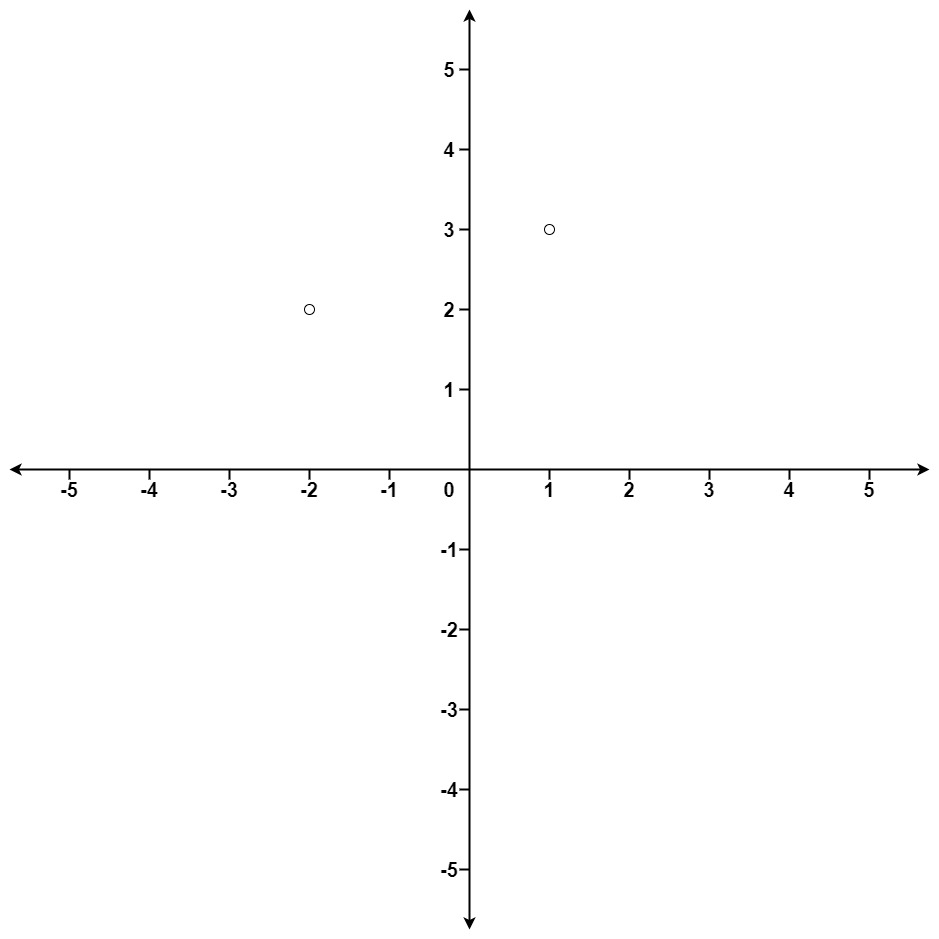
\includegraphics{35b9b79b-6d05-4e5f-bbfb-09013435ac4a.jpg}
\item
  Input: points = {[}{[}1,3{]},{[}-2,2{]}{]}, k = 1

  \begin{itemize}
  \tightlist
  \item
    Output: {[}{[}-2,2{]}{]}
  \end{itemize}
\item
  Explanation:

  \begin{itemize}
  \tightlist
  \item
    The distance between (1, 3) and the origin is sqrt(10).
  \item
    The distance between (-2, 2) and the origin is sqrt(8).
  \item
    Since sqrt(8) \textless{} sqrt(10), (-2, 2) is closer to the origin.
  \item
    We only want the closest k = 1 points from the origin, so the answer
    is just {[}{[}-2,2{]}{]}.
  \end{itemize}
\item
  Example 2:

  \begin{itemize}
  \tightlist
  \item
    Input: points = {[}{[}3,3{]},{[}5,-1{]},{[}-2,4{]}{]}, k = 2
  \item
    Output: {[}{[}3,3{]},{[}-2,4{]}{]}
  \item
    Explanation: The answer {[}{[}-2,4{]},{[}3,3{]}{]} would also be
    accepted.
  \end{itemize}
\end{itemize}

    \begin{tcolorbox}[breakable, size=fbox, boxrule=1pt, pad at break*=1mm,colback=cellbackground, colframe=cellborder]
\prompt{In}{incolor}{ }{\boxspacing}
\begin{Verbatim}[commandchars=\\\{\}]

\end{Verbatim}
\end{tcolorbox}

    \subsubsection{Q973 Psuedocode}\label{q973-psuedocode}

    \begin{tcolorbox}[breakable, size=fbox, boxrule=1pt, pad at break*=1mm,colback=cellbackground, colframe=cellborder]
\prompt{In}{incolor}{ }{\boxspacing}
\begin{Verbatim}[commandchars=\\\{\}]
\PY{k}{for} \PY{n}{point} \PY{o+ow}{in} \PY{n}{points}\PY{p}{:}
\PY{n}{Calculate} \PY{n}{squared} \PY{n}{distance} \PY{k+kn}{from} \PY{n+nn}{origin}
    \PY{n}{Push} \PY{n}{point} \PY{k}{with} \PY{n}{negative} \PY{n}{distance} \PY{n}{to} \PY{n}{maintain} \PY{n+nb}{min} \PY{n}{heap}
\PY{n}{Replace} \PY{n}{the} \PY{n}{farthest} \PY{n}{point} \PY{k}{if} \PY{n}{current} \PY{n}{point} \PY{o+ow}{is} \PY{n}{closer}
\PY{n}{Extract} \PY{n}{points} \PY{k+kn}{from} \PY{n+nn}{heap} \PY{o+ow}{and} \PY{k}{return} \PY{k}{as} \PY{n+nb}{list}
\end{Verbatim}
\end{tcolorbox}

    \subsubsection{Q973 Code.py}\label{q973-code.py}

    \begin{tcolorbox}[breakable, size=fbox, boxrule=1pt, pad at break*=1mm,colback=cellbackground, colframe=cellborder]
\prompt{In}{incolor}{7}{\boxspacing}
\begin{Verbatim}[commandchars=\\\{\}]
\PY{k+kn}{import} \PY{n+nn}{heapq}
\PY{k}{class} \PY{n+nc}{Solution}\PY{p}{:}
    \PY{k}{def} \PY{n+nf}{kClosest}\PY{p}{(}\PY{n+nb+bp}{self}\PY{p}{,} \PY{n}{points}\PY{p}{,} \PY{n}{k}\PY{p}{)}\PY{p}{:}
        \PY{n}{heap} \PY{o}{=} \PY{p}{[}\PY{p}{]}
        \PY{k}{for} \PY{n}{point} \PY{o+ow}{in} \PY{n}{points}\PY{p}{:}
            \PY{n}{distance} \PY{o}{=} \PY{n+nb}{sum}\PY{p}{(}\PY{n+nb}{map}\PY{p}{(}\PY{k}{lambda} \PY{n}{x}\PY{p}{:} \PY{n}{x} \PY{o}{*}\PY{o}{*} \PY{l+m+mi}{2}\PY{p}{,} \PY{n}{point}\PY{p}{)}\PY{p}{)}
            \PY{k}{if} \PY{n+nb}{len}\PY{p}{(}\PY{n}{heap}\PY{p}{)} \PY{o}{\PYZlt{}} \PY{n}{k}\PY{p}{:}
                \PY{n}{heapq}\PY{o}{.}\PY{n}{heappush}\PY{p}{(}\PY{n}{heap}\PY{p}{,} \PY{p}{[}\PY{o}{\PYZhy{}}\PY{n}{distance}\PY{p}{,} \PY{n}{point}\PY{p}{]}\PY{p}{)}
            \PY{k}{else}\PY{p}{:}
                \PY{k}{if} \PY{o}{\PYZhy{}}\PY{n}{distance} \PY{o}{\PYZgt{}} \PY{n}{heap}\PY{p}{[}\PY{l+m+mi}{0}\PY{p}{]}\PY{p}{[}\PY{l+m+mi}{0}\PY{p}{]}\PY{p}{:}
                    \PY{n}{heapq}\PY{o}{.}\PY{n}{heappop}\PY{p}{(}\PY{n}{heap}\PY{p}{)}
                    \PY{n}{heapq}\PY{o}{.}\PY{n}{heappush}\PY{p}{(}\PY{n}{heap}\PY{p}{,} \PY{p}{[}\PY{o}{\PYZhy{}}\PY{n}{distance}\PY{p}{,} \PY{n}{point}\PY{p}{]}\PY{p}{)}
        \PY{k}{return} \PY{p}{[}\PY{n}{point} \PY{k}{for} \PY{n}{distance}\PY{p}{,} \PY{n}{point} \PY{o+ow}{in} \PY{n}{heap}\PY{p}{]}


\PY{n}{solution} \PY{o}{=} \PY{n}{Solution}\PY{p}{(}\PY{p}{)}
\PY{n}{points} \PY{o}{=} \PY{p}{[}\PY{p}{[}\PY{l+m+mi}{1}\PY{p}{,} \PY{l+m+mi}{3}\PY{p}{]}\PY{p}{,} \PY{p}{[}\PY{o}{\PYZhy{}}\PY{l+m+mi}{2}\PY{p}{,} \PY{l+m+mi}{2}\PY{p}{]}\PY{p}{]}
\PY{n}{k} \PY{o}{=} \PY{l+m+mi}{1}
\PY{n+nb}{print}\PY{p}{(}\PY{n}{solution}\PY{o}{.}\PY{n}{kClosest}\PY{p}{(}\PY{n}{points}\PY{p}{,} \PY{n}{k}\PY{p}{)}\PY{p}{)}
\end{Verbatim}
\end{tcolorbox}

    \begin{Verbatim}[commandchars=\\\{\}]
[[-2, 2]]
    \end{Verbatim}

    \textbf{Problem4-LeetcodeQ 215. Kth Largest Element in an Array-Medium}

Given an integer array nums and an integer k, return the kth largest
element in the array.

Note that it is the kth largest element in the sorted order, not the kth
distinct element.

Can you solve it without sorting?

\begin{itemize}
\tightlist
\item
  Example 1:

  \begin{itemize}
  \tightlist
  \item
    Input: nums = {[}3,2,1,5,6,4{]}, k = 2
  \item
    Output: 5
  \end{itemize}
\item
  Example 2:

  \begin{itemize}
  \tightlist
  \item
    Input: nums = {[}3,2,3,1,2,4,5,5,6{]}, k = 4
  \item
    Output: 4
  \end{itemize}
\end{itemize}

    \subsubsection{Q215 Psuedocode}\label{q215-psuedocode}

    \begin{tcolorbox}[breakable, size=fbox, boxrule=1pt, pad at break*=1mm,colback=cellbackground, colframe=cellborder]
\prompt{In}{incolor}{ }{\boxspacing}
\begin{Verbatim}[commandchars=\\\{\}]
\PY{n}{define} \PY{n}{function} \PY{n}{maxHeapify} \PY{k}{with} \PY{n}{parameters} \PY{n}{arr} \PY{p}{(}\PY{n+nb}{list} \PY{n}{of} \PY{n}{integers}\PY{p}{)}\PY{p}{,} \PY{n}{i} \PY{p}{(}\PY{n}{integer}\PY{p}{)}\PY{p}{,} \PY{n}{end} \PY{p}{(}\PY{n}{integer}\PY{p}{)}
\PY{n+nb}{set} \PY{n}{j} \PY{n}{to} \PY{l+m+mi}{2} \PY{o}{*} \PY{n}{i} \PY{o}{+} \PY{l+m+mi}{1}
\PY{k}{while} \PY{n}{j} \PY{o+ow}{is} \PY{n}{less} \PY{n}{than} \PY{o+ow}{or} \PY{n}{equal} \PY{n}{to} \PY{n}{end}
    \PY{k}{if} \PY{n}{j} \PY{o}{+} \PY{l+m+mi}{1} \PY{o+ow}{is} \PY{n}{less} \PY{n}{than} \PY{o+ow}{or} \PY{n}{equal} \PY{n}{to} \PY{n}{end} \PY{o+ow}{and} \PY{n}{arr}\PY{p}{[}\PY{n}{j} \PY{o}{+} \PY{l+m+mi}{1}\PY{p}{]} \PY{o+ow}{is} \PY{n}{greater} \PY{n}{than} \PY{n}{arr}\PY{p}{[}\PY{n}{j}\PY{p}{]}
        \PY{n}{increment} \PY{n}{j} \PY{n}{by} \PY{l+m+mi}{1}
    \PY{k}{if} \PY{n}{arr}\PY{p}{[}\PY{n}{i}\PY{p}{]} \PY{o+ow}{is} \PY{n}{less} \PY{n}{than} \PY{n}{arr}\PY{p}{[}\PY{n}{j}\PY{p}{]}
        \PY{n}{swap} \PY{n}{arr}\PY{p}{[}\PY{n}{i}\PY{p}{]} \PY{o+ow}{and} \PY{n}{arr}\PY{p}{[}\PY{n}{j}\PY{p}{]}
        \PY{n+nb}{set} \PY{n}{i} \PY{n}{to} \PY{n}{j}
        \PY{n+nb}{set} \PY{n}{j} \PY{n}{to} \PY{l+m+mi}{2} \PY{o}{*} \PY{n}{i} \PY{o}{+} \PY{l+m+mi}{1}
    \PY{k}{else}
        \PY{k}{break}

\PY{n+nb}{set} \PY{n}{n} \PY{n}{to} \PY{n}{the} \PY{n}{length} \PY{n}{of} \PY{n}{nums}
\PY{k}{for} \PY{n}{i} \PY{k+kn}{from} \PY{n+nn}{n} \PY{o}{/}\PY{o}{/} \PY{l+m+mi}{2} \PY{o}{\PYZhy{}} \PY{l+m+mi}{1} \PY{n}{down} \PY{n}{to} \PY{l+m+mi}{0} \PY{p}{(}\PY{n}{inclusive}\PY{p}{)}
    \PY{n}{call} \PY{n}{maxHeapify} \PY{k}{with} \PY{n}{nums}\PY{p}{,} \PY{n}{i}\PY{p}{,} \PY{o+ow}{and} \PY{n}{n} \PY{o}{\PYZhy{}} \PY{l+m+mi}{1}

\PY{k}{for} \PY{n}{j} \PY{k+kn}{from} \PY{n+nn}{n} \PY{o}{\PYZhy{}} \PY{l+m+mi}{1} \PY{n}{down} \PY{n}{to} \PY{n}{n} \PY{o}{\PYZhy{}} \PY{n}{k} \PY{p}{(}\PY{n}{inclusive}\PY{p}{)}
    \PY{n}{swap} \PY{n}{nums}\PY{p}{[}\PY{l+m+mi}{0}\PY{p}{]} \PY{o+ow}{and} \PY{n}{nums}\PY{p}{[}\PY{n}{j}\PY{p}{]}
    \PY{n}{call} \PY{n}{maxHeapify} \PY{k}{with} \PY{n}{nums}\PY{p}{,} \PY{l+m+mi}{0}\PY{p}{,} \PY{o+ow}{and} \PY{n}{j} \PY{o}{\PYZhy{}} \PY{l+m+mi}{1}

\PY{k}{return} \PY{n}{nums}\PY{p}{[}\PY{o}{\PYZhy{}}\PY{n}{k}\PY{p}{]}
\end{Verbatim}
\end{tcolorbox}

    \subsubsection{Q215 Code.py}\label{q215-code.py}

    \begin{tcolorbox}[breakable, size=fbox, boxrule=1pt, pad at break*=1mm,colback=cellbackground, colframe=cellborder]
\prompt{In}{incolor}{8}{\boxspacing}
\begin{Verbatim}[commandchars=\\\{\}]
\PY{k+kn}{from} \PY{n+nn}{typing} \PY{k+kn}{import} \PY{n}{List}

\PY{k}{class} \PY{n+nc}{Solution}\PY{p}{:}
    \PY{k}{def} \PY{n+nf}{findKthLargest}\PY{p}{(}\PY{n+nb+bp}{self}\PY{p}{,} \PY{n}{nums}\PY{p}{:} \PY{n}{List}\PY{p}{[}\PY{n+nb}{int}\PY{p}{]}\PY{p}{,} \PY{n}{k}\PY{p}{:} \PY{n+nb}{int}\PY{p}{)} \PY{o}{\PYZhy{}}\PY{o}{\PYZgt{}} \PY{n+nb}{int}\PY{p}{:}
        \PY{k}{def} \PY{n+nf}{maxHepify}\PY{p}{(}\PY{n}{arr}\PY{p}{,} \PY{n}{i}\PY{p}{,} \PY{n}{end}\PY{p}{)}\PY{p}{:}     
            \PY{n}{j} \PY{o}{=} \PY{l+m+mi}{2} \PY{o}{*} \PY{n}{i} \PY{o}{+} \PY{l+m+mi}{1}                 
            \PY{k}{while} \PY{n}{j} \PY{o}{\PYZlt{}}\PY{o}{=} \PY{n}{end}\PY{p}{:}             
                \PY{k}{if} \PY{n}{j} \PY{o}{+} \PY{l+m+mi}{1} \PY{o}{\PYZlt{}}\PY{o}{=} \PY{n}{end} \PY{o+ow}{and} \PY{n}{arr}\PY{p}{[}\PY{n}{j} \PY{o}{+} \PY{l+m+mi}{1}\PY{p}{]} \PY{o}{\PYZgt{}} \PY{n}{arr}\PY{p}{[}\PY{n}{j}\PY{p}{]}\PY{p}{:}   
                    \PY{n}{j} \PY{o}{+}\PY{o}{=} \PY{l+m+mi}{1}                              
                \PY{k}{if} \PY{n}{arr}\PY{p}{[}\PY{n}{i}\PY{p}{]} \PY{o}{\PYZlt{}} \PY{n}{arr}\PY{p}{[}\PY{n}{j}\PY{p}{]}\PY{p}{:}             
                    \PY{n}{arr}\PY{p}{[}\PY{n}{i}\PY{p}{]}\PY{p}{,} \PY{n}{arr}\PY{p}{[}\PY{n}{j}\PY{p}{]} \PY{o}{=} \PY{n}{arr}\PY{p}{[}\PY{n}{j}\PY{p}{]}\PY{p}{,} \PY{n}{arr}\PY{p}{[}\PY{n}{i}\PY{p}{]}     
                    \PY{n}{i} \PY{o}{=} \PY{n}{j}                       
                    \PY{n}{j} \PY{o}{=} \PY{l+m+mi}{2} \PY{o}{*} \PY{n}{i} \PY{o}{+} \PY{l+m+mi}{1}                 
                \PY{k}{else}\PY{p}{:}                           
                    \PY{k}{break}
        
        \PY{n}{n} \PY{o}{=} \PY{n+nb}{len}\PY{p}{(}\PY{n}{nums}\PY{p}{)}
        \PY{k}{for} \PY{n}{i} \PY{o+ow}{in} \PY{n+nb}{range}\PY{p}{(}\PY{n}{n} \PY{o}{/}\PY{o}{/} \PY{l+m+mi}{2} \PY{o}{\PYZhy{}} \PY{l+m+mi}{1}\PY{p}{,} \PY{o}{\PYZhy{}}\PY{l+m+mi}{1}\PY{p}{,} \PY{o}{\PYZhy{}}\PY{l+m+mi}{1}\PY{p}{)}\PY{p}{:} 
            \PY{n}{maxHepify}\PY{p}{(}\PY{n}{nums}\PY{p}{,} \PY{n}{i}\PY{p}{,} \PY{n}{n} \PY{o}{\PYZhy{}} \PY{l+m+mi}{1}\PY{p}{)}

        \PY{k}{for} \PY{n}{j} \PY{o+ow}{in} \PY{n+nb}{range}\PY{p}{(}\PY{n}{n} \PY{o}{\PYZhy{}} \PY{l+m+mi}{1}\PY{p}{,} \PY{n}{n} \PY{o}{\PYZhy{}} \PY{n}{k} \PY{o}{\PYZhy{}} \PY{l+m+mi}{1}\PY{p}{,} \PY{o}{\PYZhy{}}\PY{l+m+mi}{1}\PY{p}{)}\PY{p}{:}
            \PY{n}{nums}\PY{p}{[}\PY{l+m+mi}{0}\PY{p}{]}\PY{p}{,} \PY{n}{nums}\PY{p}{[}\PY{n}{j}\PY{p}{]} \PY{o}{=} \PY{n}{nums}\PY{p}{[}\PY{n}{j}\PY{p}{]}\PY{p}{,} \PY{n}{nums}\PY{p}{[}\PY{l+m+mi}{0}\PY{p}{]}    
            \PY{n}{maxHepify}\PY{p}{(}\PY{n}{nums}\PY{p}{,} \PY{l+m+mi}{0}\PY{p}{,} \PY{n}{j} \PY{o}{\PYZhy{}} \PY{l+m+mi}{1}\PY{p}{)}               
        
        \PY{k}{return} \PY{n}{nums}\PY{p}{[}\PY{o}{\PYZhy{}}\PY{n}{k}\PY{p}{]}


\PY{n}{nums} \PY{o}{=} \PY{p}{[}\PY{l+m+mi}{3}\PY{p}{,} \PY{l+m+mi}{2}\PY{p}{,} \PY{l+m+mi}{1}\PY{p}{,} \PY{l+m+mi}{5}\PY{p}{,} \PY{l+m+mi}{6}\PY{p}{,} \PY{l+m+mi}{4}\PY{p}{]}
\PY{n}{k} \PY{o}{=} \PY{l+m+mi}{2}
\PY{n}{solution} \PY{o}{=} \PY{n}{Solution}\PY{p}{(}\PY{p}{)}
\PY{n+nb}{print}\PY{p}{(}\PY{n}{solution}\PY{o}{.}\PY{n}{findKthLargest}\PY{p}{(}\PY{n}{nums}\PY{p}{,} \PY{n}{k}\PY{p}{)}\PY{p}{)}  \PY{c+c1}{\PYZsh{} Output should be 5}
\end{Verbatim}
\end{tcolorbox}

    \begin{Verbatim}[commandchars=\\\{\}]
5
    \end{Verbatim}

    \begin{tcolorbox}[breakable, size=fbox, boxrule=1pt, pad at break*=1mm,colback=cellbackground, colframe=cellborder]
\prompt{In}{incolor}{ }{\boxspacing}
\begin{Verbatim}[commandchars=\\\{\}]

\end{Verbatim}
\end{tcolorbox}


    % Add a bibliography block to the postdoc
    
    
    
\end{document}
